\documentclass{report}
\usepackage[utf8]{inputenc}
\usepackage{graphicx}
\usepackage{float}
\title{Process Book:Visualisation}
\author{Aniraj Kesavan and Ashwini Janamatti}
\begin{document}
\maketitle
\chapter{Proposal}
We will do a set of visualisations about various aspects of movies released and documented over time from the IMDb Database.\\
We'll primarily be relying on a curated dataset of 5000 movies.\\
Start of the visualisation will include a timelapse showing a cloud of all the movies recorded.\\
There will be a slider for showing the time lapse which will interact with movie cloud. Once you finalise on an year, it will show a bunch of visualisations for the year.\\

\section{Background and Motivation}
We were interested in showing the evolution of movies. A timelapse of a series 
of images will help do that. We were also interested in the best way to visualise 
deeper statistics of data. We did find contextual navigation to be very useful.
For instance, if you research movie names in google, it will also show you suggestions on search results of the actors associated with it. We wanted to extend
the idea using a complex data set that was available to us. We will curate an existing dataset from IMDB to realise the visualisation

\section{Project Objectives}
We would like to learn how to do contextual visualisation. We also plan to learn how to make a transition involving complex objects and possibily come up with an algorithm for drawing navigation (lines) that doesn't interfere with regular elements.

\section{Data}
We'll be using a curated dataset of 5000 movies extracted from imdb. \\
The data will have a lot of dimensions. Most important ones are the following
\begin{itemize}
\item Movie Title
\item Director Name
\item Gross Boxoffice Collection
\item Budget
\item Genre
\item Keywords
\item Duration
\item Primary Actor
\item Primary Actress
\item Facebook likes for the movie page
\item Facebook likes for the director
\item Facebook likes for Actor1, Actor2 etc
\end{itemize}
\section{Visualisation Design}
\section{Must Have Visualisations}
\subsubsection{Per year Visualisation}
\begin{itemize}
\item{\textbf{Main Tab}}
There will be a main tab of visualisation for every year. Once you slide the slider to the corresponding set of years, it'll stabilise the view and arrange the charts. Main Page There are three different navigations from the main page.
Key elements in this page are Highest Grossing Movies of the year which is an interactive bar chart. It shows top 10 moveies which are scrollable to show more and when clicked on it, it will go to an overlay boxoffice tab\\\\
There is a tile chart of movies that are sorted by a metric (eg: Most popular), the metric is toggleable to other metrics (eg: Most rating, most facebook likes) etc That is selected from a drop down. Clicking on any movie will update the movie detail pane\\

\begin{figure}[H]
	\centering{
		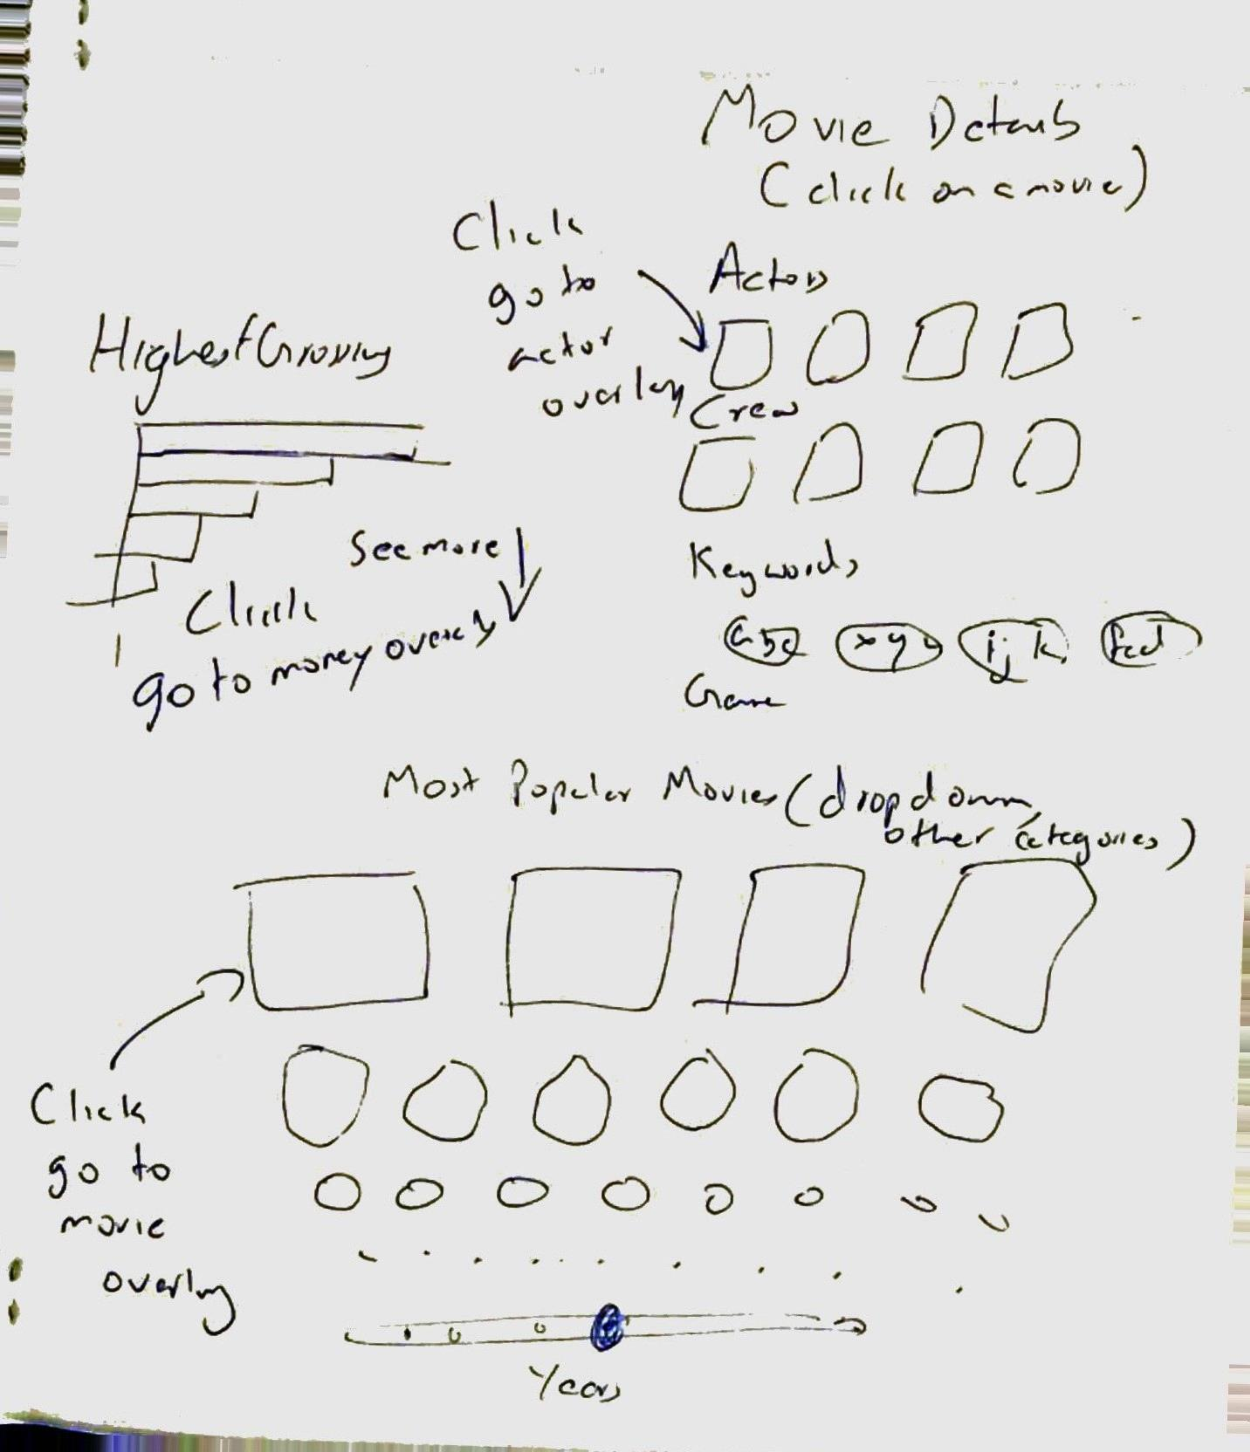
\includegraphics[width=.9\linewidth]{year_sketch_1}
	}
	\caption{Main Page. You can see the Movie Pane and the tiles. These would be per year}
	\label{Fig:1}
\end{figure}

\item{\textbf{Movie Detail Pane}}
Movie detail pane will have tiles showing actors/ other crew members and keywords and genre associated with it. Clicking on a person will take you the Personal Overlay tab and Clicking on the genre/keyword will take you to a tab showing list of movies that have similar keywords or fall under the same genre.\\\\
\item{\textbf{Navigation Tabs}}
Clicking on actor/director will get you the personal overlay tab, you can come back to the previous tab or navigate elsewhere\\\\
\begin{figure}[H]
	\centering{
		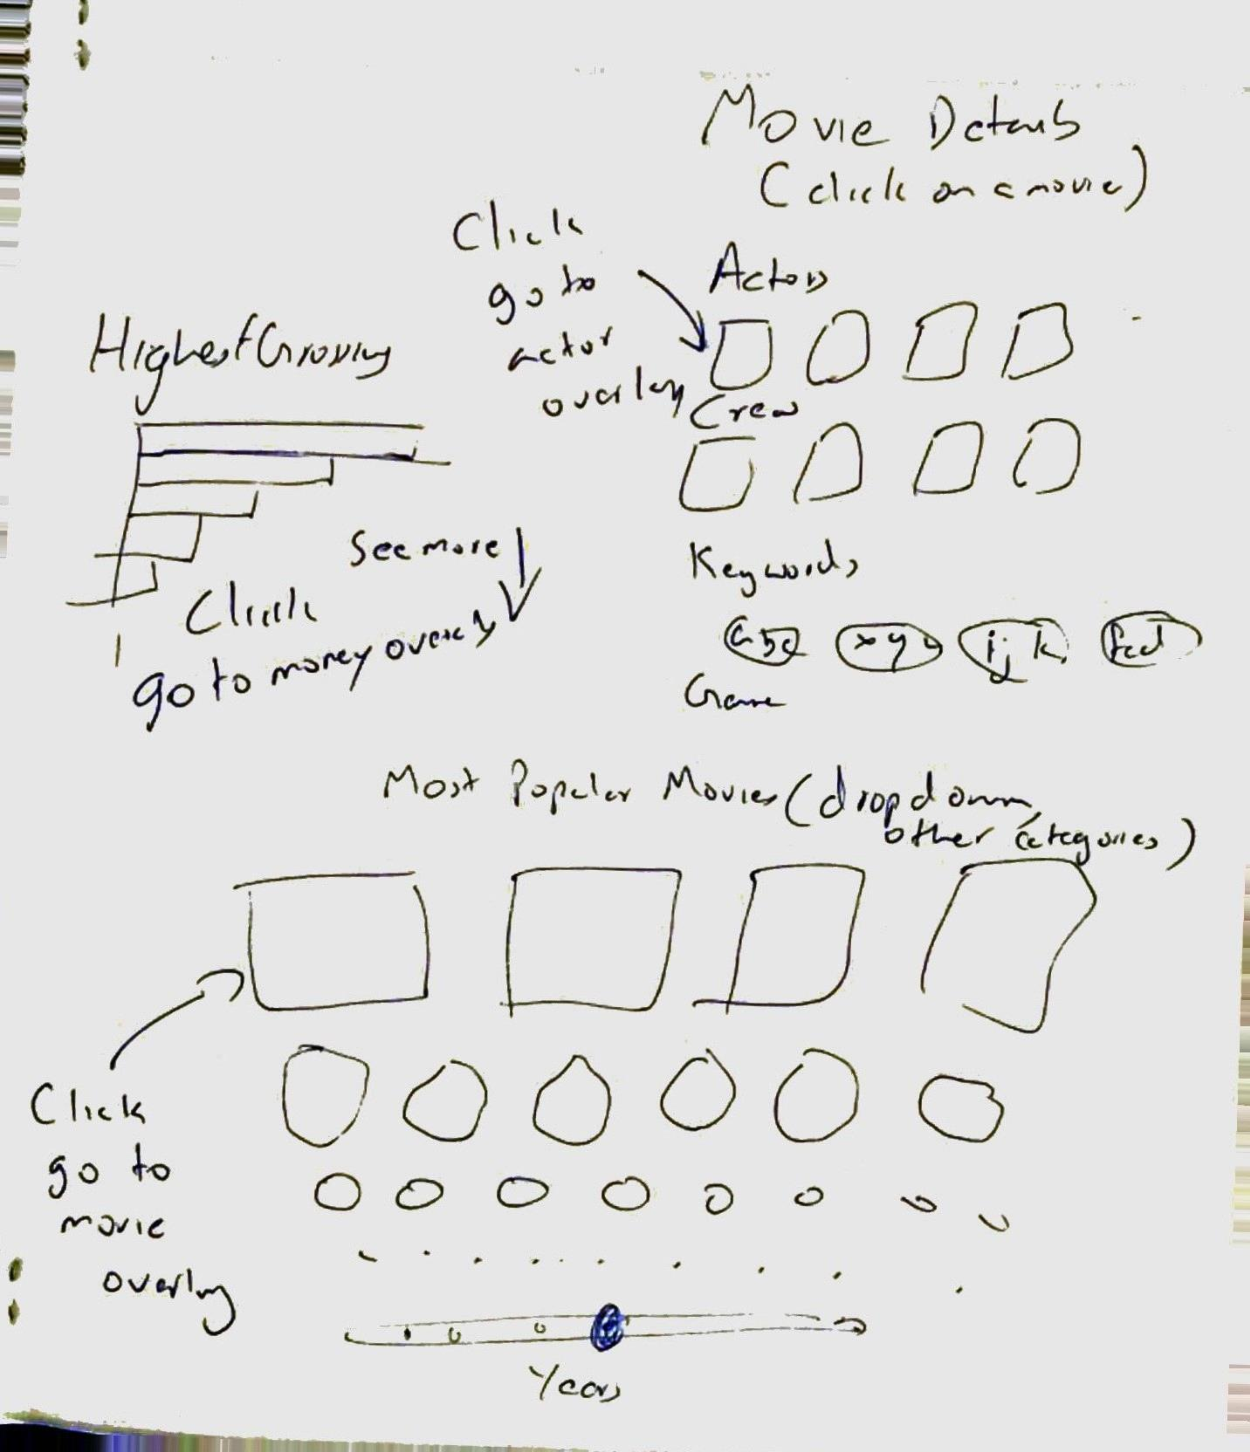
\includegraphics[width=.9\linewidth]{year_sketch_1}
	}
	\caption{Two possible overlay tabs. One showing the personell details and another for keywords/genre}
	\label{Fig:2}
\end{figure}

\end{itemize}


\section{Additional Features}
\subsubsection{Animated Movie Cloud}
Start of the visualisation will include a timelapse showing a cloud of all the movies recorded.\\
The timelapse could be an additional feature and clean demarcation of lines are definitely additional features.
\subsubsection{Additional Navigation Tabs}
Clicking on Genre/Keyword of a movie will show you to Similar movies overlay tab which similar movies in a seperate tab which can navigate to the main page with the selected movie\\\\
Clicking on the boxoffice bar will take you the show you similar grossing movies as well as movies with a similar budget as well as a details pane for the current movie. you can navigate to main page again clicking on a movie\\\\
\begin{figure}[H]
	\centering{
		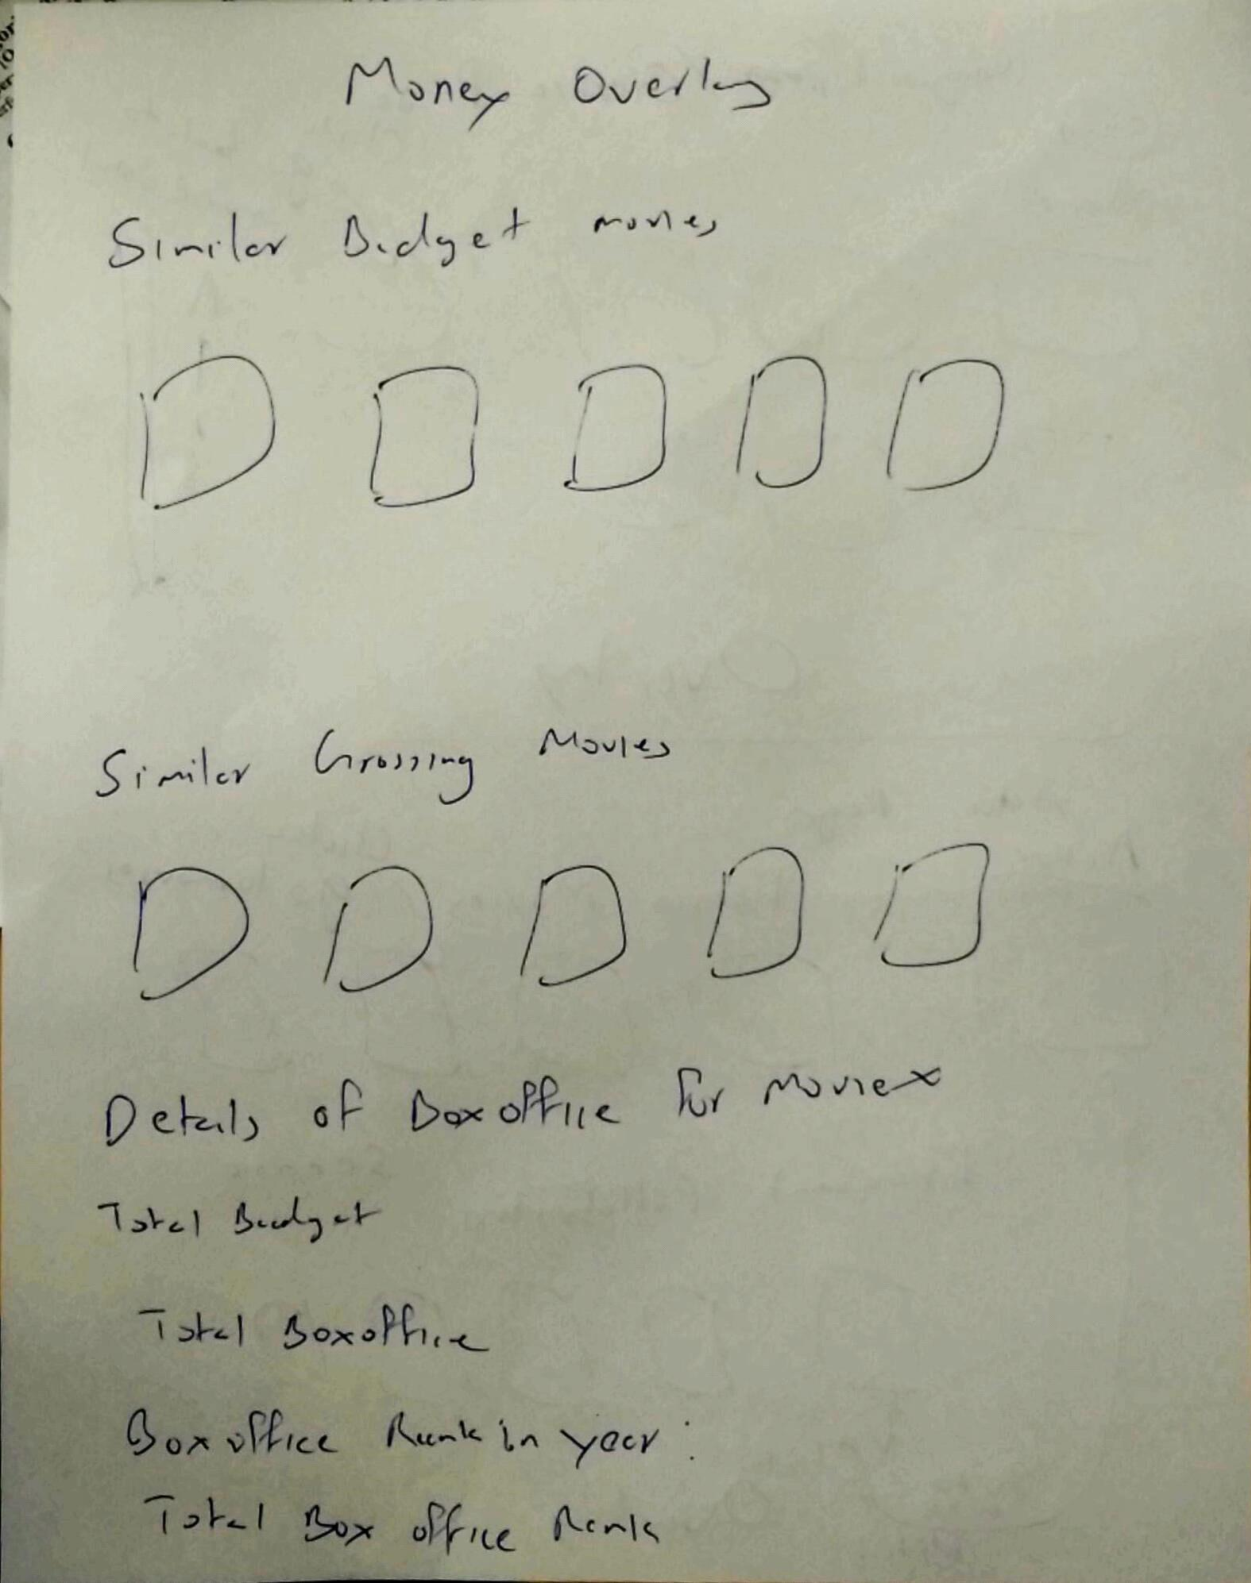
\includegraphics[width=.9\linewidth]{year_sketch_2}
	}
	\caption{Money Overlay Tab.}
	\label{Fig:3}
\end{figure}

\section{Project Schedule}
\begin{itemize}
\item November 11th: Get the dataset ready, start work on templates of tabs and timelapse
\item November 24th: Work on basic timelapse complete, navigation tabs ready
\item December 1st: Navigations complete
\item December 2nd: Polishing complete.
\end{itemize}

\section{Feedback}
These were the key ideas from the feedback provided by Stefan Hamilton and Anil Dhungel
\begin{enumerate}
\item Objectives are interesting, especially linking between various objects in panes and timelapse
\item Scope is too large, move most of it to additional features.
\item Design seems scalable
\item Primary encoding: Size of pictures/nodes. 
\item Other visual variables: Links between nodes and other items. 
Colours could be used for genre/keywords.
\item Interaction is responsive 
\item Views are coordinated within the timelapse and the navigation tab but not integrated together.
\item Timelapse animation(big bang) during page load might not fit well.
\end{enumerate}
\section{List of Figures}
A list of figures from the brainstorming sessions and the peer feedback session are attached in Chapter ~\ref{chap-milestone1}.\\


The first figure is the animation timelapse and how it might look like, you can see how each elements interact and how the transitions might look like.\\


Second figure is the main tab in the visualisation, It contains the movie detail pane, the highest grossing movies chart and a sorted tile chart of movies based on various criteria.\\


Third figure is the money overlay tab and similar grossing movies. it also shows a detail pane that will rank all money related aspects of the selected movie.\\

Fourth figure shows the overlay tabs for persons (Actor/Director) as well as the overlay tab for the genre/keyword. It's shown how the similar movies to the genre as well as frequent collaborators and their famous movies to the actor are displayed in this overlay tab.\\

Final figure is a scanned copy of the peer feedback we received in the feedback session\\

\chapter{MileStone 1}
\label{chap-milestone1}
\section{Progress}
We finalised designs for the timelapse and implemented a strawman version of it.
We also finalised the layouts for navigation tabs for other pages.
Attaching the three designs we went through for timelapse
\begin{figure}[H]
	\centering{
		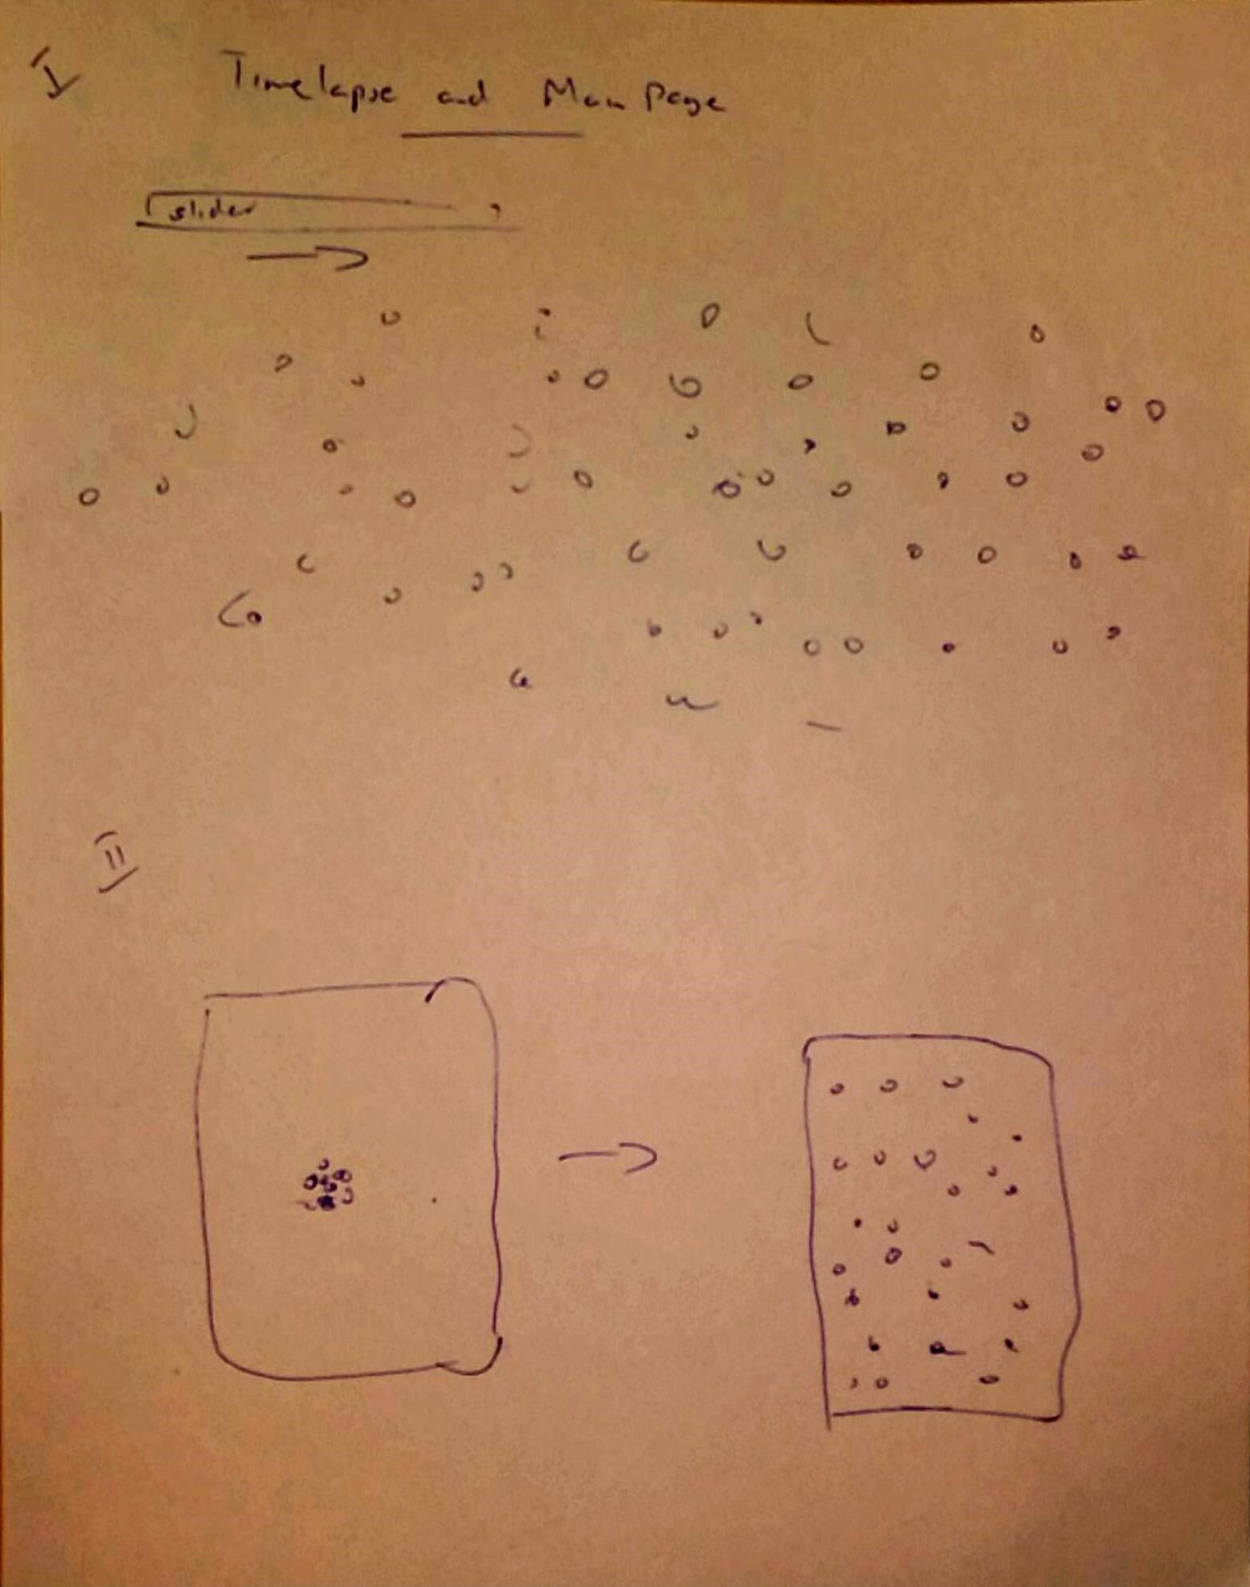
\includegraphics[width=.6\linewidth]{timelapse_1}
	}
	\caption{Timelapse Designs I and II}
	\label{Fig:4}
\end{figure}
\begin{figure}[H]
	\centering{
		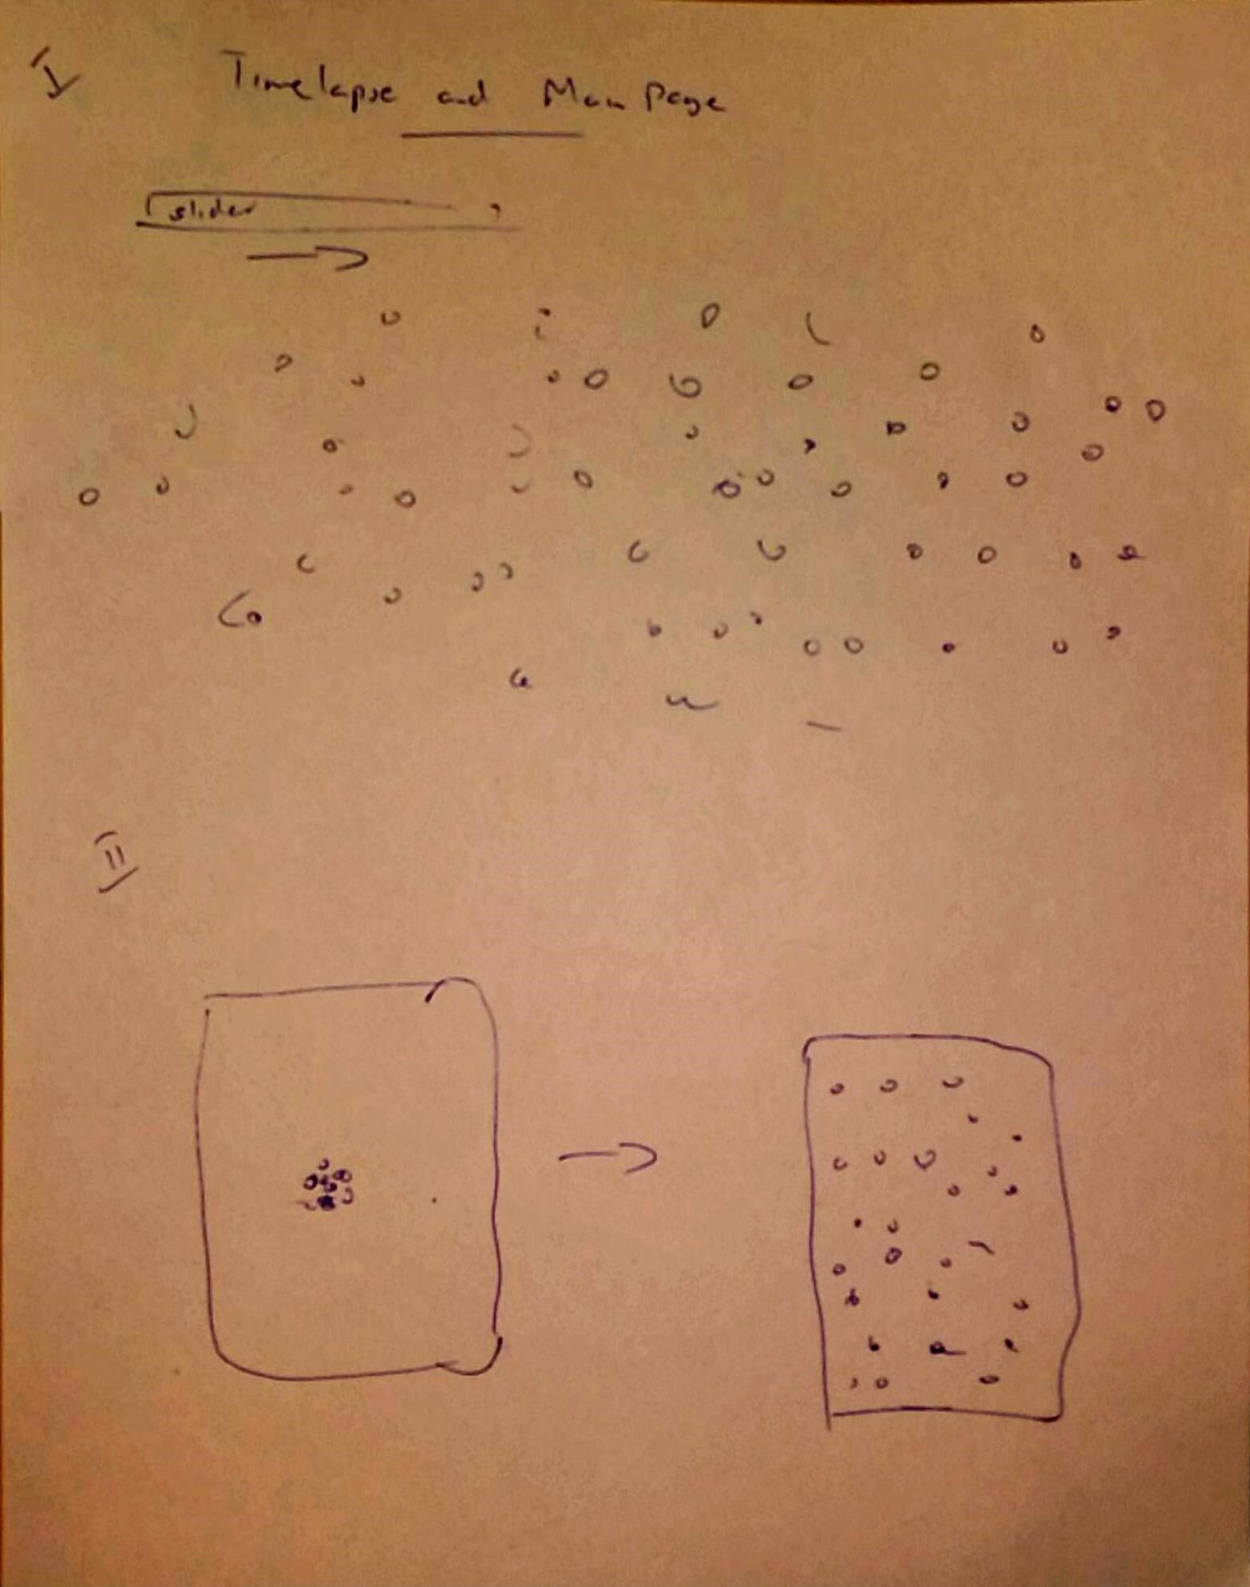
\includegraphics[width=.6\linewidth]{timelapse_1}
	}
	\caption{Timelapse Design III}
	\label{Fig:5}
\end{figure}

We have implemented a basic looking timelapse with a forcebody animation in script.js in the repository.


\end{document}

